%%%%%%%%%%%%%%%%%%%%%%%%%%%%%%%%%%%%%%%%%%%%%%%%%%%%%%%%%%%%%%%%%%%%
%
%   Style for CMS Computing / Physics Technical Design Reports
%
%   Lucas Taylor  4 Feb 2005,   Revised  12 Oct 2005
%
%%%%%%%%%%%%%%%%%%%%%%%%%%%%%%%%%%%%%%%%%%%%%%%%%%%%%%%%%%%%%%%%%%%%

%  the following line is edited by the tdr script to change or to pass
%  additional options:
\documentclass[11pt,twoside,a4paper,an]{cms-tdr}
\def\svnVersion{489401}

%%%%%%%%%%%%%%%%%%%%%%%%%%%%%%%%%%%%%%%%%%%%%%%%%%%%%%%%%%%%%%%%%%%%

\begin{document}
%%%%%%%%%%%%%%%%%%%%%%%%%%%%%%%%%%%%%%%%%%%%%%%%%%%%%%%%%%%%%%%%%%%%
%
%  Common definitions
%
%  N.B. use of \providecommand rather than \newcommand means
%       that a definition is ignored if already specified
%
%                                              L. Taylor 18 Feb 2005
%%%%%%%%%%%%%%%%%%%%%%%%%%%%%%%%%%%%%%%%%%%%%%%%%%%%%%%%%%%%%%%%%%%%


%%%%%%%%%%%%%%%%%%%%%%%%%%%%%%%%%%%%%%%%%%%%%%%%%%%%%%%%%%%%%%%%%%%%
%
% Hyphenations (only need to add here if you get a nasty word break)
%
\hyphenation{had-ron-i-za-tion}
\hyphenation{cal-or-i-me-ter}
\hyphenation{de-vices}
%
% Hyphenations-end
% % Customizable fields and text areas start with % >> below.
% Lines starting with the comment character (%) are normally removed before release outside the collaboration, but not those comments ending lines

% svn info. These are modified by svn at checkout time.
% The last version of these macros found before the maketitle will be the one on the front page,
% so only the main file is tracked.
% Do not edit by hand!
\RCS$Revision: 481969 $
\RCS$HeadURL: svn+ssh://svn.cern.ch/reps/tdr2/notes/AN-18-239/trunk/AN-18-239.tex $
\RCS$Id: AN-18-239.tex 481969 2018-11-21 15:19:49Z michgall $
%%%%%%%%%%%%% local definitions %%%%%%%%%%%%%%%%%%%%%
% This allows for switching between one column and two column (cms@external) layouts
% The widths should  be modified for your particular figures. You'll need additional copies if you have more than one standard figure size.
\newlength\cmsFigWidth
\ifthenelse{\boolean{cms@external}}{\setlength\cmsFigWidth{0.49\textwidth}}{\setlength\cmsFigWidth{0.65\textwidth}} % example: one column in journal, 2/3 in CMS
\ifthenelse{\boolean{cms@external}}{\providecommand{\cmsLeft}{upper\xspace}}{\providecommand{\cmsLeft}{left\xspace}}
\ifthenelse{\boolean{cms@external}}{\providecommand{\cmsRight}{lower\xspace}}{\providecommand{\cmsRight}{right\xspace}}

\newcommand{\exctlob}{pp\rightarrow pp 2\ell1b\xspace}


%%%%%%%%%%%%%%%  Title page %%%%%%%%%%%%%%%%%%%%%%%%
\cmsNoteHeader{AN-18-239} % This is over-written in the CMS environment: useful as preprint no. for export versions
% >> Title: please make sure that the non-TeX equivalent is in PDFTitle below
\title{Searching for exclusively produced top quark pairs}

% >> Authors
%Author is always "The CMS Collaboration" for PAS and papers, so author, etc, below will be ignored in those cases
%For multiple affiliations, create an address entry for the combination
%To mark authors as primary, use the \author* form
\address[cern]{CERN, Geneva, Switzerland}
\address[lip]{LIP, Laborat\'{o}rio de Instrumenta\c{c}\~{a}o e F\'{i}sica Experimental de Part\'{i}culas, Lisbon, Portugal}
\author[lip]{B.~Ribeiro Lopes}
\author[cern]{P.~Silva}
\author[lip]{J.~Hollar}
\author[lip]{M.~Gallinaro}


% >> Date
% The date is in yyyy/mm/dd format. Today has been
% redefined to match, but if the date needs to be fixed, please write it in this fashion.
% For papers and PAS, \today is taken as the date the head file (this one) was last modified according to svn: see the RCS Id string above.
% For the final version it is best to "touch" the head file to make sure it has the latest date.
\date{\today}

% >> Abstract
% Abstract processing:
% 1. **DO NOT use \include or \input** to include the abstract: our abstract extractor will not search through other files than this one.
% 2. **DO NOT use %**                  to comment out sections of the abstract: the extractor will still grab those lines (and they won't be comments any longer!).
% 3. For PASs: **DO NOT use tex macros**         in the abstract: CDS MathJax processor used on the abstract doesn't understand them _and_ will only look within $$. The abstracts for papers are hand formatted so macros are okay.
\abstract{
A search for exclusive production of top quark pairs, where the outgoing unfragmented protons are detected about 210~m away from the centre of the CMS detector, is described. 
Proton-proton collision data at $\sqrt{s}=$13~TeV collected in 2017 are used for the search. An upper limit is set on the production cross section.
}

% >> PDF Metadata
% Do not comment out the following hypersetup lines (metadata). They will disappear in NODRAFT mode and are needed by CDS.
% Also: make sure that the values of the metadata items are sensible and are in plain text:
% (1) no TeX! -- for \sqrt{s} use sqrt(s) -- this will show with extra quote marks in the draft version but is okay).
% (2) no %.
% (3) No curly braces {}.
\hypersetup{%
pdfauthor={B. Ribeiro Lopes$^a$, P. Ferreira da Silva$^{a,b}$, J. Hollar$^b$, M. Gallinaro$^a$},%
pdftitle={Searching for exclusively produced top quark pairs},%
pdfsubject={CMS},%
pdfkeywords={CMS, physics, top quark, exclusive production, PPS}}

\maketitle %maketitle comes after all the front information has been supplied
% >> Text
%%%%%%%%%%%%%%%%%%%%%%%%%%%%%%%%  Begin text %%%%%%%%%%%%%%%%%%%%%%%%%%%%%
%% **DO NOT REMOVE THE BIBLIOGRAPHY** which is located before the appendix.
%% You can take the text between here and the bibiliography as an example which you should replace with the actual text of your document.
%% If you include other TeX files, be sure to use "\input{filename}" rather than "\input filename".
%% The latter works for you, but our parser looks for the braces and will break when uploading the document.
%%%%%%%%%%%%%%%

%\author{B. Ribeiro Lopes$^a$, P. Ferreira da Silva$^{a,b}$, J. Hollar$^b$, M. Gallinaro$^a$}



\tableofcontents
\newpage
%
%
%
\section{Introduction}
\label{sec:intro}

This note reports on the search for exclusive top quark pairs, $pp\rightarrow p\ttbar p$, 
where the $\ttbar$ pair decays dileptonically. The process is represented by the Feynman diagrams in Fig.~\ref{feynman}.
If identified in the data, this production channel is characterized by the suppression
of additional radiation in the central region.
If the kinematics of the protons are measured, it offers the possibility of determining the \ttbar{} production threshold with a better resolution than the one that can be attained based on the inclusive production, through the reconstruction of the final states.
The standard model (SM) prediction for the exclusive top pair production cross section is extremely small, $\mathcal{O}({\rm 1~fb})$ for photo-production, and it lacks updated predictions~\cite{deFavereaudeJeneret:2009db}.
However, if new physics is present, the small cross section can be significantly enhanced either in the production of \ttbar{} or in the production of similar final states containing at least two leptons~\cite{Bussey:2006vx,Heinemeyer:2008sb,TaheriMonfared:2014pya,Piotrzkowski:2009sa}.

In our analysis, the two leptons (electrons or muons) and the b-jets from the top quark decay are measured in the central CMS apparatus, while the two outgoing protons are measured in the Precision Proton Spectrometer (PPS). The latter is a near-beam magnetic spectrometer that uses the LHC magnets between the Interaction Point (IP) and detector stations at $\approx\pm$210 m from the IP. Protons that have lost a small fraction of their momentum are bent out of the beam envelope so that their trajectories can be measured. The detectors that form PPS are called Roman Pots (RPs).

\begin{figure}[!htp]
\centering
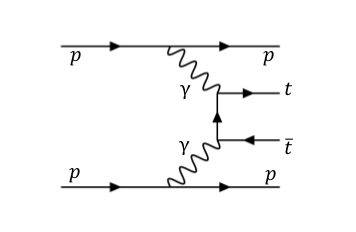
\includegraphics[width=0.49\textwidth]{figures/feynman1.png}
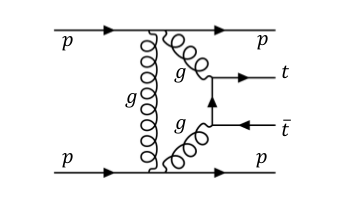
\includegraphics[width=0.49\textwidth]{figures/feynman2.png}
\caption{Exclusive $\ttbar$ production diagrams, via $\gamma \gamma$ fusion (left) and $gg$ fusion (right).}
\label{feynman}
\end{figure}

%
%
%
\section{Data and simulation samples}
\label{sec:samples}

The analysis is performed using proton-proton collision data at $\sqrt{s}=13$ TeV collected in 2017. The SingleMuon and SingleElectron primary datasets (PDs) are used\footnote{These are chosen as the starting point for the analysis, but could be complemented in a future version with the DoubleElectron, DoubleMuon and MuEG datasets to maximize the efficiency for the dilepton final state.}. The events passing the triggers listed on Table~\ref{tab:triggers} are considered in our analysis. 
The total integrated luminosity corresponds to 41.4 fb$^{-1}$.

\begin{table}[!htp]
\begin{center}
\caption{Triggers used in the selection of the events. Events where both the muon and one of the electron trigger fires are allowed only if they are found in the SingleMuon PD.}
\label{tab:triggers}
\begin{tabular}{ l }
\hline\hline
Trigger name \\
\hline
HLT\_Ele35\_eta2p1\_WPTight\_Gsf\_v* \\ 
HLT\_Ele28\_eta2p1\_WPTight\_Gsf\_HT150\_v* \\
HLT\_Ele30\_eta2p1\_WPTight\_Gsf\_CentralPFJet35\_EleCleaned\_v* \\
HLT\_IsoMu27\_v \\
\hline\hline
\end{tabular}
\end{center}
\end{table}

For the correlation between the central detector and the PPS, only data collected before Technical Stop 2 (TS2) are used. This is because both the detector efficiency and the PPS acceptance (due to new LHC optics) are different after-TS2 data and their measurement is still being finalized. 
In the PPS, RPs are identified followed by a 3-digit number, where the first digit is either 0 or 1 according to which arm the pot belongs to (0 for a positive z coordinate: z+, and 1 for negative z coordinate: z-), the second digit is the station number (either 0 for strips, or 2 for pixels), and the third is the RP number.
RP numbered 003 and 103 contain silicon strip detectors, while those labeled 023 and 123 contain 3D pixel detectors. The scheme of the PPS detector and its arms is shown in Fig.~\ref{fig:pps}.
Only data from RPs 003, 023, 103 and 123 were used, since no alignment parameters exist for other RPs. Besides, only collisions with crossing angle of 120, 130 or 140 $\mu$rad are considered, because there are no dispersion values available for other crossing angles.
The total integrated luminosity where combined CMS(central)-PPS data have been analysed with calibrated pixels is thus reduced to 18.7~fb$^{-1}$.

\begin{figure}[!htp]
\centering
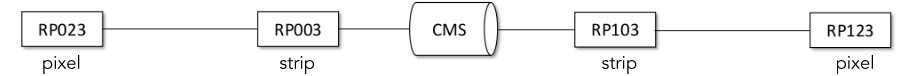
\includegraphics[width=.9\textwidth]{figures/pps.png}
\caption{Scheme of the PPS detectors used in the analysis.}
\label{fig:pps}
\end{figure}

The official Monte Carlo production samples have been used for the background. The name of the samples and the cross section used to normalize them is summarized in Table~\ref{tab:mc}.

\begin{table}[!htp]
\begin{center}
\caption{MC samples from the
RunIIFall17MiniAOD-94X\_mc2017\_realistic\_v10
production used in this analysis and their cross section.}
\label{tab:mc}
\hspace*{-1cm}
\begin{tabular}{ lcl }
\hline\hline
Process & $\sigma$ [pb] & MC sample  \\
\hline
\ttbar & 832 & TTJets\_TuneCP5\_13TeV-amcatnloFXFX-pythia8\\
ZZ$\rightarrow 2\ell2\nu$ & 0.564 & ZZTo2L2Nu\_13TeV\_powheg\_pythia8\\
WZ & 47.13 & WZ\_TuneCP5\_13TeV-pythia8\\
WW$\rightarrow 2\ell2\nu$ & 12.178 & WWTo2L2Nu\_NNPDF31\_TuneCP5\_13TeV-powheg-pythia8\\
W+3~jets & 942.3 & W3JetsToLNu\_TuneCP5\_13TeV-madgraphMLM-pythia8\\
W+4~jets & 524.2 & W4JetsToLNu\_TuneCP5\_13TeV-madgraphMLM-pythia8\\
$\bar{t}$W & 35.85 & ST\_tW\_antitop\_5f\_NoFullyHadronicDecays\_TuneCP5\_13TeV-powheg-pythia8 \\
tW & 35.85 & ST\_tW\_top\_5f\_NoFullyHadronicDecays\_TuneCP5\_13TeV-powheg-pythia8 \\
DY (M$>$50\GeV) &  5765.4 & DYJetsToLL\_M-50\_TuneCP5\_13TeV-amcatnloFXFX-pythia8\\
\hline\hline
\end{tabular}
\end{center}
\end{table}

In addition, a signal $pp\rightarrow p\gamma\gamma p\rightarrow p \ttbar p$ sample was produced privately using \textsc{FPMC}~\cite{Boonekamp:2011ky} as the matrix element generator and \textsc{Herwig++}~\cite{Bahr:2008pv} as the parton shower. This sample is used to compute the acceptance and guide the final event selection.

%
%
%
\section{Event selection}
\label{sec:evsel}

%%
%%
%%
\subsection{Central detector selection}
\label{subsec:centralsel}

Two charged leptons (electron or muon) with $M_{\ell\ell}>20$\GeV are required. 
At least one of the leptons is required to have $\pt>30$\GeV, while the second one is required to have $\pt>15$\GeV. Both leptons are required to be reconstructed within $|\eta|<2.5$.
Depending on the flavour and invariant mass of the dilepton system,
the events are classified in the following exclusive categories:

\begin{itemize}
    \item same-flavour leptons ($ee$ or $\mu \mu$) with reconstructed $m_{\ell\ell}$ around the Z mass ($m_{\ell\ell}\in[76,106]$~\GeV): Z-control region (CR);
    \item same-flavour (SF) leptons outside the Z-peak region: SF region;
    \item opposite-flavour (OF) leptons ($e\mu$): OF region.
\end{itemize}

After categorizing the events, the following selection is applied:

\begin{itemize}
    \item $\geq$ 1 jet ($\pt>20$\GeV, $|\eta|<4.7$ passing a ``loose'' pileup jet id criteria~\cite{twiki:pujetid});
    \item $\geq$ 1 b-jet ($\pt>30$\GeV, $|\eta|<2.5$ passing the deepCSV ``medium'' working point~\cite{Sirunyan:2017ezt});
    \item at least one ``lepton-b~jet" combination satisfies $M_{\ell b} < 160$\GeV.
\end{itemize}

In the last requirement, $m_{\ell b}$ refers to the invariant mass of lepton-b~jet system. All lepton-b~jet combinations are used and the one with the smallest $m_{\ell b}$ value is considered 
for the final selection. The criterion stems from the fact that, by energy conservation, one expects at leading order (LO), that $m_{\ell b}<\sqrt{m_t^2-m_W^2}\approx 160$\GeV for $m_t=172.5$\GeV and $m_W=80.4$\GeV~\cite{Tanabashi:2018oca}. Thus, by applying such requirement, we expect that higher $\ttbar$ purity is attained.

Figure~\ref{mll} shows the distribution of the invariant mass of the dilepton system for the SF and OF categories. It can be observed that even after removing the Z-peak region, the SF category is expected to be dominated by the Drell-Yan (DY) production. The excess in data for $m_{\ell\ell}<50$\GeV is expected given the DY simulation does not include that region. For the OF category an overall excess is observed which may be attributed to missing simulated processes (to be checked).

\begin{figure}[!htp]
\centering
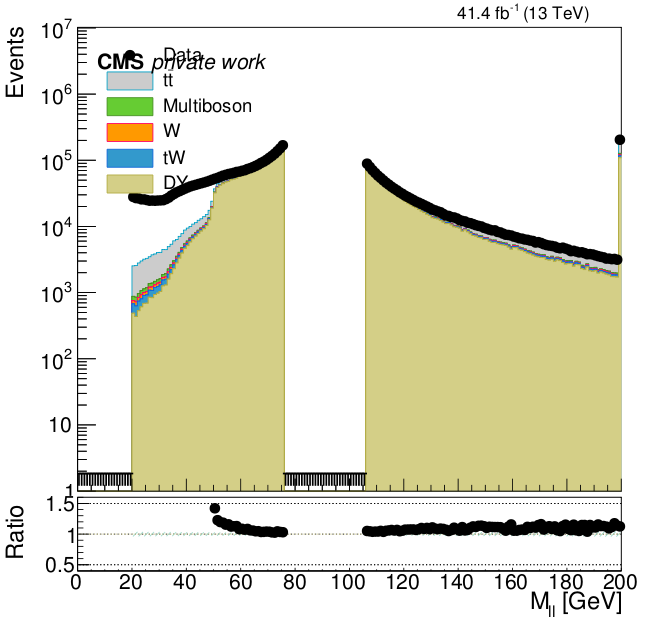
\includegraphics[width=.49\textwidth]{figures/2lep_SF_mll_cen_log.png}
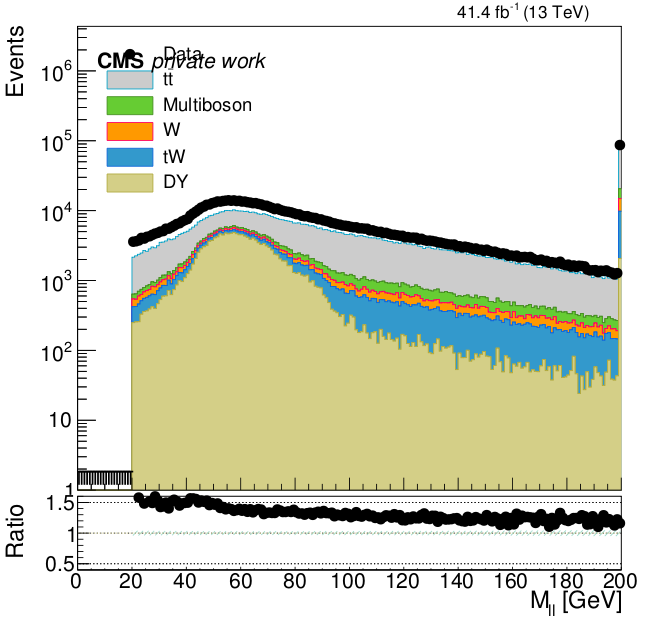
\includegraphics[width=.49\textwidth]{figures/2lep_OF_mll_cen_log.png}
\caption{Control sample (central detector only): Distribution of the mass of the dilepton system after selecting two leptons for same-flavour (SF) leptons for events outside the Z peak (left), and for opposite-flavour leptons (right). Data are compared to the stacked predictions based on the simulation. The bottom panels show the ratio of the data to the total expected predictions.}
\label{mll}
\end{figure}

Figure~\ref{nbjets} shows the distribution of the b-tagging multiplicity. An excess is observed for events with low multiplicity in both the SF and OF categories. The excess disappears once the high purity region of $\ttbar$ is selected ($\geq 1$ b-tag).

\begin{figure}[!htp]
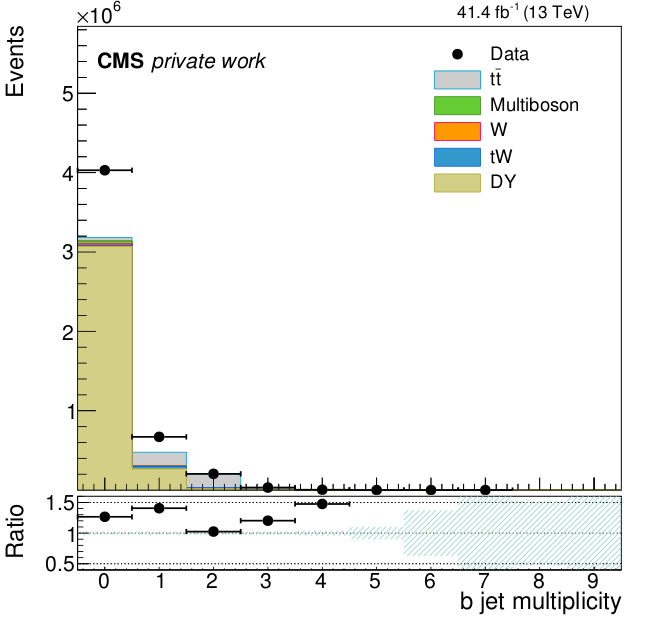
\includegraphics[width=.49\textwidth]{figures/2lep_SF_nbjets.png}
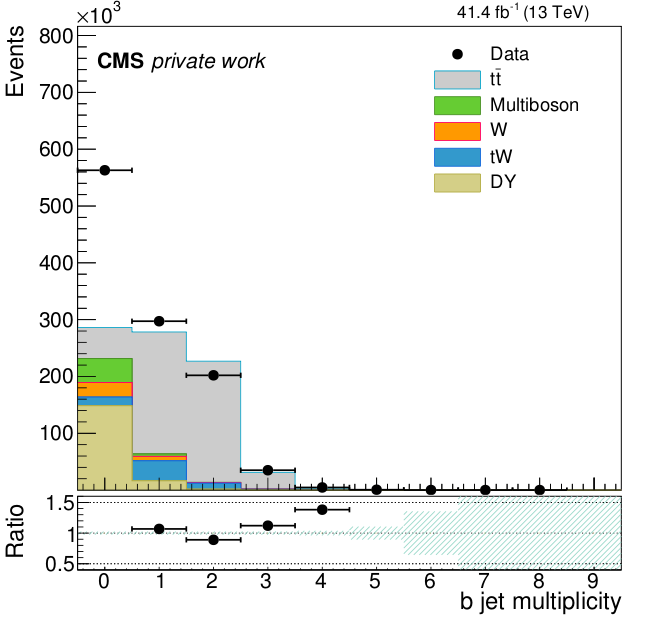
\includegraphics[width=.49\textwidth]{figures/2lep_OF_nbjets.png}
\caption{Control sample (central detector only): Number of b-tagged jets after requiring 2 leptons, for same flavour leptons except events under the Z peak (left) and for opposite flavour leptons (right).}
\label{nbjets}
\end{figure}

Figure~\ref{Mlb} shows the distribution of the $m_{\ell b}$ variable after the selection of at least 1 b-jet.
An overall excess for the high $m_{\ell b}$ region is observed in both the SF and OF categories. This may be due to missing simulated samples (to be confirmed). In any case these events are removed from our analysis as the low $m_{\ell b}$ region ($m_{\ell b}<160\GeV$) is the one which is expected to be enriched in \ttbar{} events.

\begin{figure}[!htp]
\centering
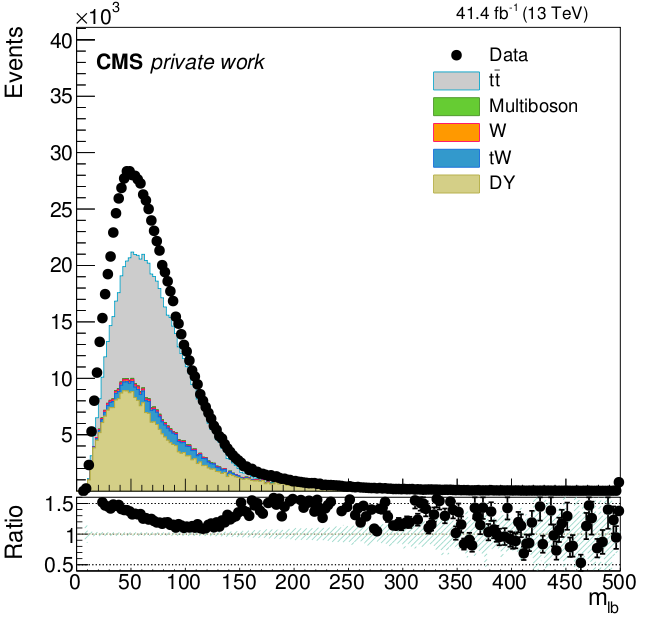
\includegraphics[width=.49\textwidth]{figures/1b_SF_Mlb.png}
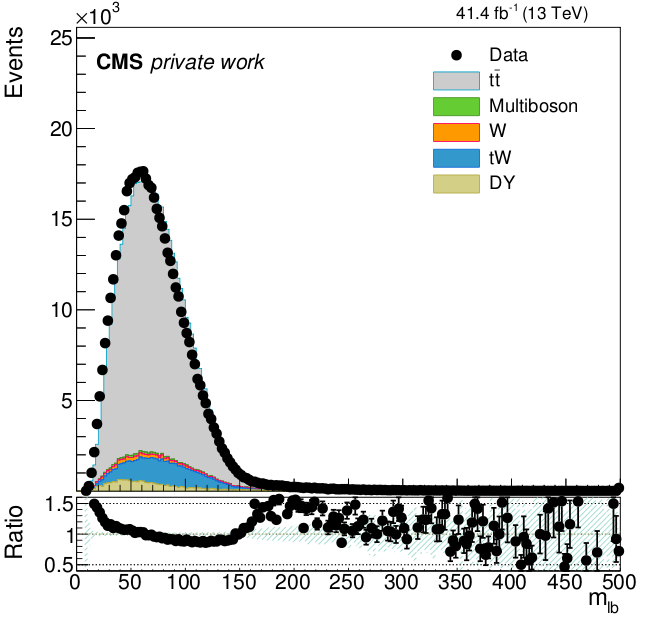
\includegraphics[width=.49\textwidth]{figures/1b_OF_Mlb.png}
\caption{Control sample (central detector only): Mass of the lepton/b-jet system, after requiring two leptons, one jet and one b-jet, for same-flavour (SF) leptons in events outside the Z peak region (left), and for opposite-flavour (OF) leptons (right).}
\label{Mlb}
\end{figure}

We compare exclusive (signal) and inclusive (background) \ttbar{} samples with respect to specific variables reconstructed in the central detector. The variables are chosen as they are sensitive to the additional hadronic activity, which is expected to be suppressed in the case the production is exclusive and via electroweak vertices. The variables chosen are:

\begin{itemize}
\item $H_T=\sum_{j=1}^{N_j} |\vec{p}_{\rm T,j}|$, the scalar sum of the transverse momentum of all jets except for the b-jets;
\item Hadronic recoil $h=|\vec{p}_T^{miss}+\vec{p}_T(\ell_1)+\vec{p}_T(\ell_2)+\sum_{j=1}^{N_b}\vec{p}_T(j)|$, obtained from the sum of the missing transverse energy with the two charged leptons and up to two b-jets.  In the analysis we make use of the so-called puppiMET estimator for $\vec{p}_T^{miss}$~\cite{CMS-PAS-JME-17-001}.
\end{itemize}

In the simulation, we observe that in the exclusive \ttbar{} sample (signal) most of the events have little ``extra activity", that is most of the events have $H_T$=0 given there are no extra jets in the events. In addition, exclusive \ttbar{} events tend to have lower $h$ when compared to inclusive \ttbar production. 
Figure~\ref{hvars} shows the distributions of these variables in data and simulation. A slight disagreement is observed with respect to the predictions, but no systematic uncertainties (\eg related to pileup, and jet energy scale) are shown at this point.

\begin{figure}[!htp]
\centering
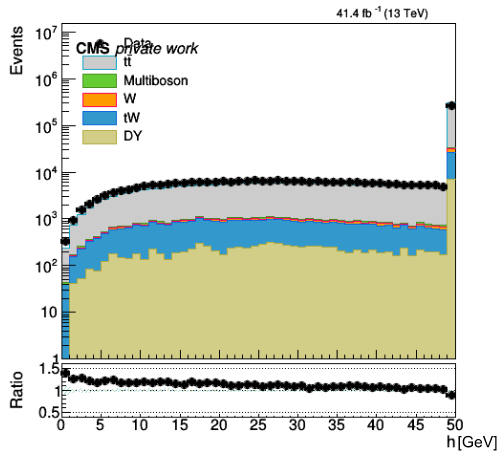
\includegraphics[width=0.49\textwidth]{figures/h.png}
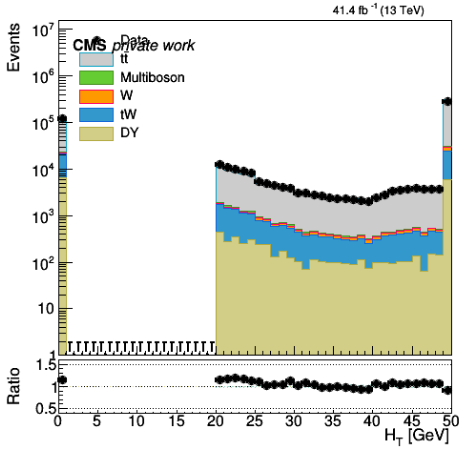
\includegraphics[width=0.49\textwidth]{figures/ht.png}
\caption{Control sample (central detector only): Hadronic activity distributions obtained after requiring 2 opposite-flavour (OF) leptons, 1 jet, 1 b-jet, $m_{\ell b}<$160\GeV. 
Distributions of the hadronic recoil $h$ (left) and $H_T$ (right) are shown (see text).}
\label{hvars}
\end{figure}

A comparison between distributions in exclusive (signal) and inclusive (background) $\ttbar$ events is furthermore performed for the two important hadronic activity variables. 
Figure~\ref{hvars_mc} shows that the observed difference is significant between the two \ttbar{} production mechanisms. This information can be used to purify the event selection.
In this analysis we require that $H_T=0$ GeV in the signal region.

\begin{figure}[!htp]
\centering
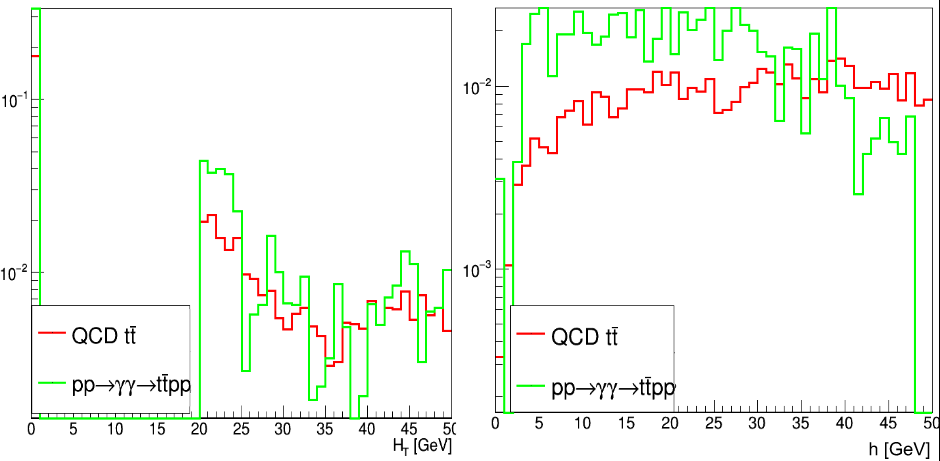
\includegraphics[width=.8\linewidth]{figures/h_ht.png}
\caption{Control sample (central detector only): distributions of $H_T$ (left) and $h$ (right) for exclusive (signal) and inclusive (background) $\ttbar$ events.
Distributions are normalized to unity.}
\label{hvars_mc}
\end{figure}



\subsection{PPS detector selection}
\label{subsec:ppssel}

For the final selection, we use data from the pixel detectors. The choice for using the RP instrumented with the pixels is made as pixels can reconstruct more than one track per event and, in case of pileup, the signal is not lost due to reconstruction inefficiency.
For each track reconstructed in the pixel detector it is possible to reconstruct the fractional proton momentum loss ($\xi$). 
The $\xi$ distribution for each pixel is shown in Fig.~\ref{xi}, for a fraction of the dataset.

\begin{figure}[!htp]
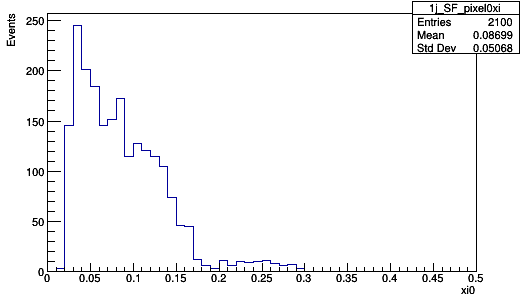
\includegraphics[width=.49\textwidth]{figures/xi0.png}
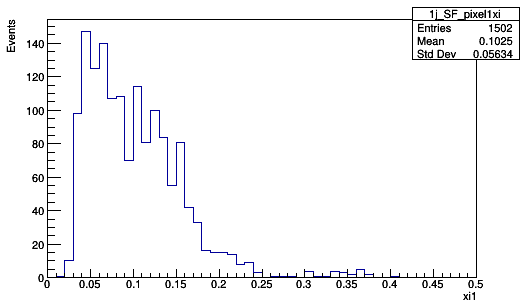
\includegraphics[width=.49\textwidth]{figures/xi1.png}
\caption{Distribution of the fractional momentum loss ($\xi$) of the protons detected in the pixels, for RP023 (left) and RP123 (right) (only a fraction of the dataset is used here).}
  \label{xi}
\end{figure}

From the values of $\xi_0$ (for z+) and $\xi_1$ (for z-) one reconstructs the mass and rapidity of the $\ttbar$ from the two protons in the RPs, using the following equations:

\begin{equation}
    m_{RP} = \sqrt{s\cdot \xi_0 \cdot \xi_1} ~~~ {\rm and}~~~ y_{RP} = \frac{1}{2}\ln\left(\frac{\xi_0}{\xi_1}\right),
%
%    M_{RP} = \sqrt{s\cdot \xi_0 \cdot \xi_1}
    \label{eq:mrp}
%\end{equation}
%
%\begin{equation}
%    y_{RP} = \frac{1}{2}\ln\left(\frac{\xi_0}{\xi_1}\right)~~,
%    \label{eq:yrp}
\end{equation}

where the subscripts 0 and 1 refer to the arm index.

Due to pileup (the average vertex multiplicity in the 2017 data is $\sim$30), there is often more than one track per event in each pixel detector. 
Thus there is the need to reconstruct the mass and rapidity for every combination of tracks. 
Distributions of mass and rapidity are shown in Fig.~\ref{mRP_yRP} after requiring two leptons in the events.

\begin{figure}[!htp]
\centering
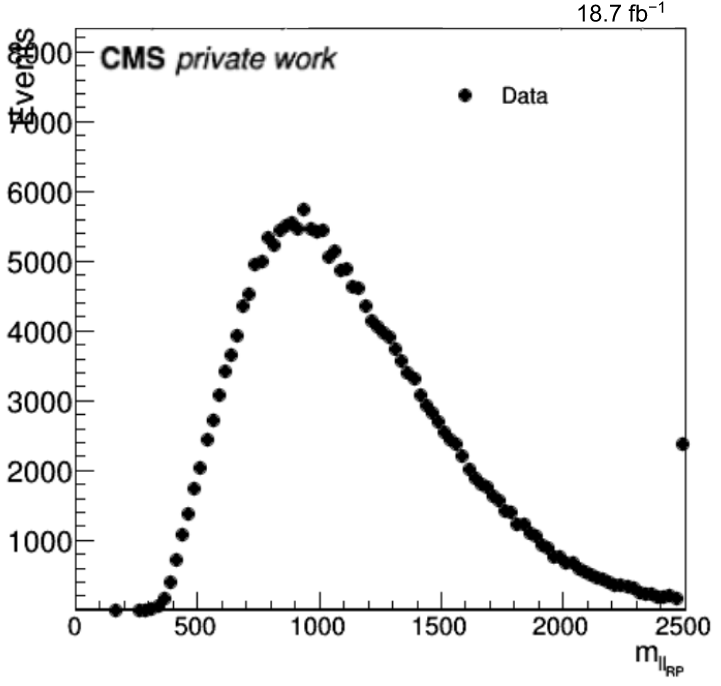
\includegraphics[width=.49\textwidth]{figures/m_rp.png}
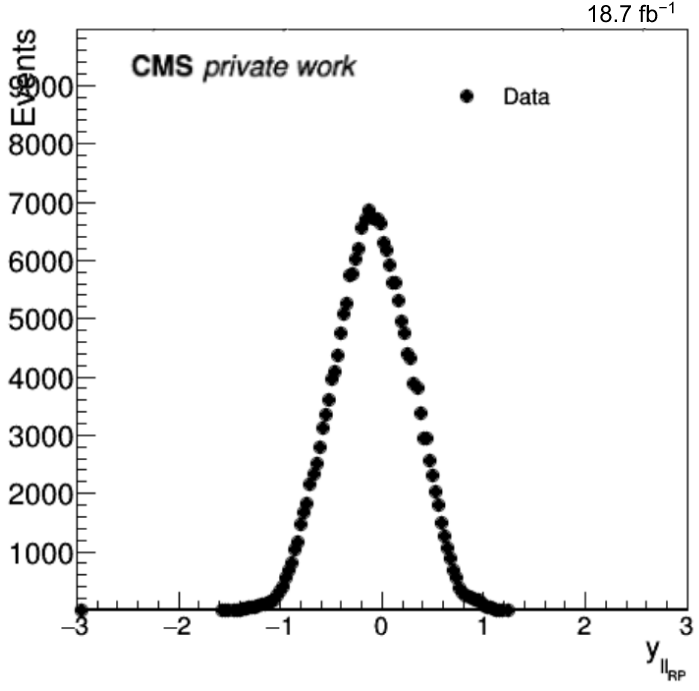
\includegraphics[width=.49\textwidth]{figures/y_rp.png}
\caption{Distributions of the reconstructed mass (left) and rapidity (right) of the dilepton system in the RPs, when requiring two opposite flavour (OF) leptons.}
\label{mRP_yRP}
\end{figure}

\begin{figure}[!htp]
\centering
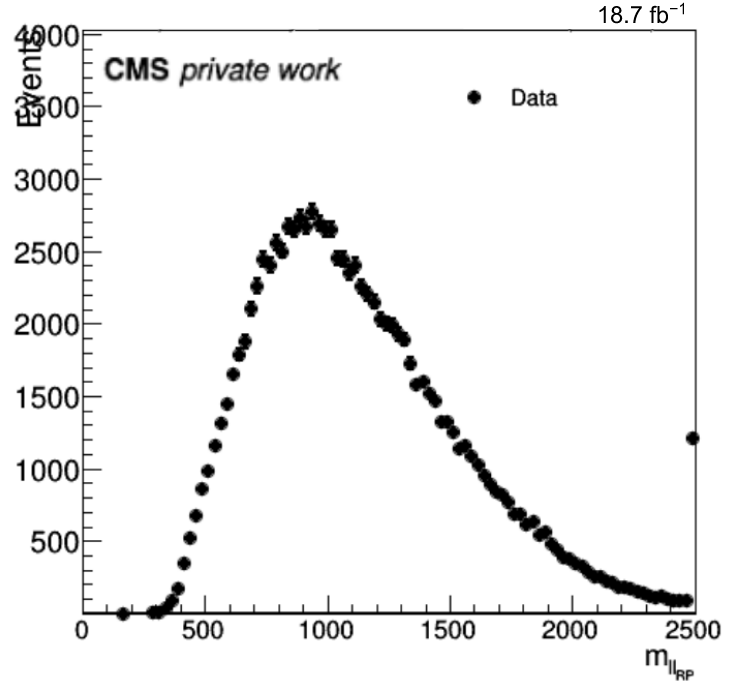
\includegraphics[width=.49\textwidth]{figures/m_rp_sel.png}
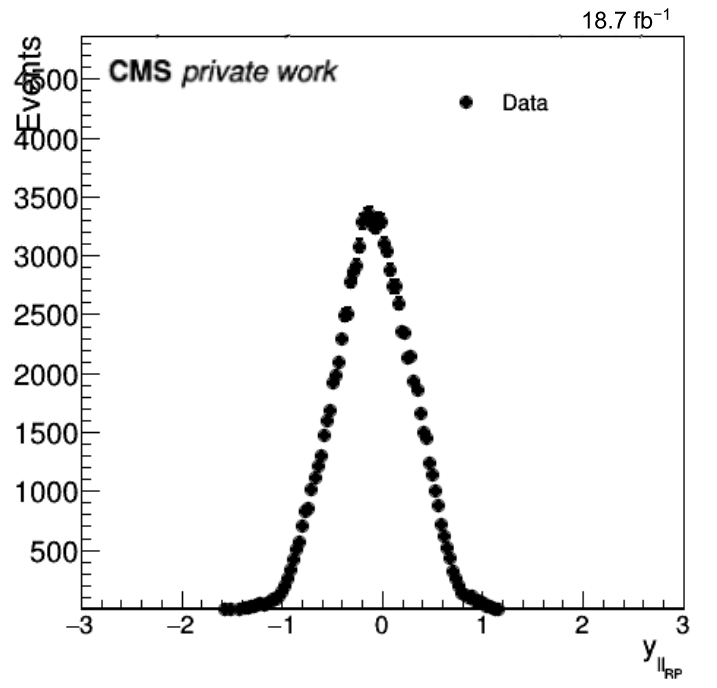
\includegraphics[width=.49\textwidth]{figures/y_rp_sel.png}
\caption{Distributions of the reconstructed mass (left) and rapidity (right) of the dilepton system in the RPs, 
when requiring 2 opposite-flavour (OF) leptons, 1 jet, 1 b-jet, low mass of the lepton/b-jet system ($M_{\ell b}<160\GeV$).}
\label{mRP_yRP_sel}
\end{figure}

In this analysis, we select events in the $m_{RP}\in[300,600]$\GeV range, chosen to be compatible with the bulk of the production threshold of exclusive $\ttbar$ events. 
Events are categorized depending on whether or not there is a combination of tracks that leads to a reconstructed \ttbar mass in this range. This is discussed in the following Section.


\subsection{Matching the central and the forward kinematics}
\label{subsec:recentral}

A further improvement in the signal-to-background (S/B) ratio may be achieved by matching the kinematics of the events reconstructed in the central and in the PPS detectors.
We apply the algorithm described in~\cite{1305.1878} to reconstruct the kinematics of the central system for the selected events. The algorithm is applied to the events which pass the full event selection described earlier. Given the ambiguity in the pairing of the leptons and the b-jets, and to the kinematics of the two outgoing neutrinos, up to 8 solutions can be found per event. 
We choose the solution that yields the lowest $m_\ttbar$.
After this choice, the mass and rapidity values computed from the forward tracks are then compared with those reconstructed using the central system. 
The correlation between $m_{RP}$ and $y_{RP}$ is shown in Fig.~\ref{rec_kinematics}.
At this point no correlation is observed, \ie the selected region is still largely dominated by inclusive $\ttbar$ events and pileup combinatorial background in the RPs. 
Figure~\ref{rec_kinematics_sim} shows the same correlation for simulated exclusive \ttbar~events. 
We can see that for the rapidity the reconstruction performs quite well, and that is not the case for the correlation in the mass distributions. 

\begin{figure}[!htp]
\centering
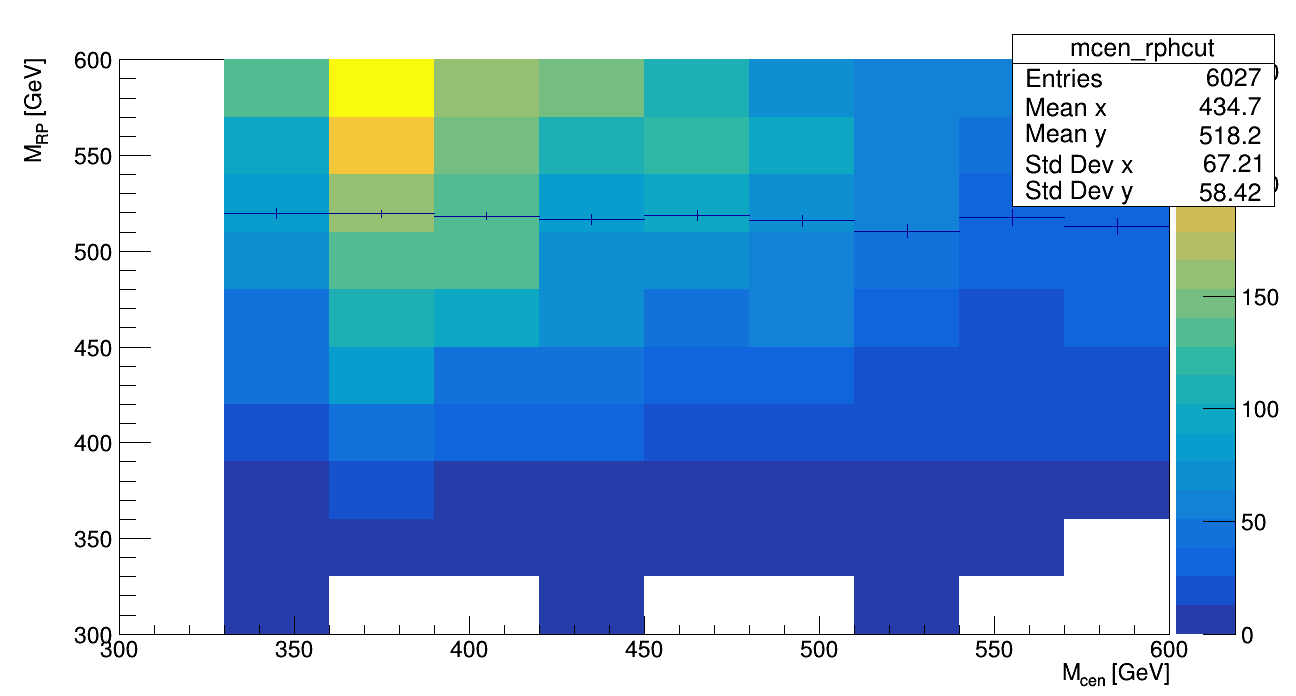
\includegraphics[width=.8\textwidth]{figures/mass_algorithm.png}\\
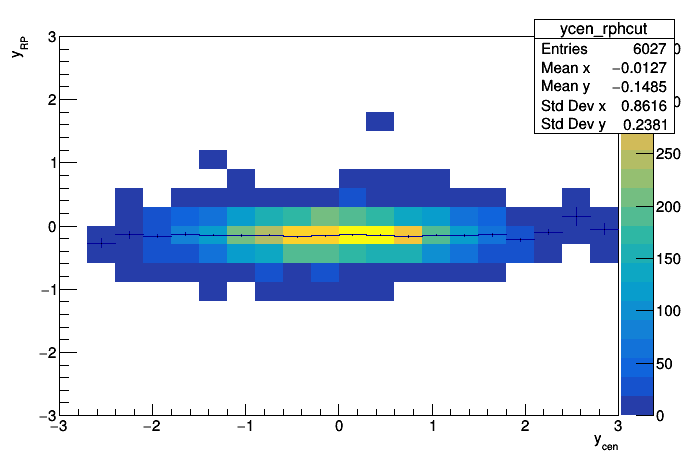
\includegraphics[width=.8\textwidth]{figures/ycen_rp.png}
\caption{
%\FIXME{to clarify ...} 
Distributions of the mass (top) and rapidity (bottom) of the dilepton \ttbar system as reconstructed using the algorithm in Ref.~\cite{1305.1878} (see text). 
%for the selected events in the central detector ($m_{cen}$, $y_{cen}$) versus those reconstructed from the RP tracks ($m_{RP}$, $y_{RP}$). 
2D distributions are shown for the selected events reconstructed in the central detector ($m_{cen}$, $y_{cen}$) versus the values reconstructed from the RP tracks ($m_{RP}$, $y_{RP}$).
%
The profile of each distribution is overlaid. The black cross centers at the mean and the bars indicate the standard deviation.}
\label{rec_kinematics}
\end{figure}

\begin{figure}[!htp]
\centering
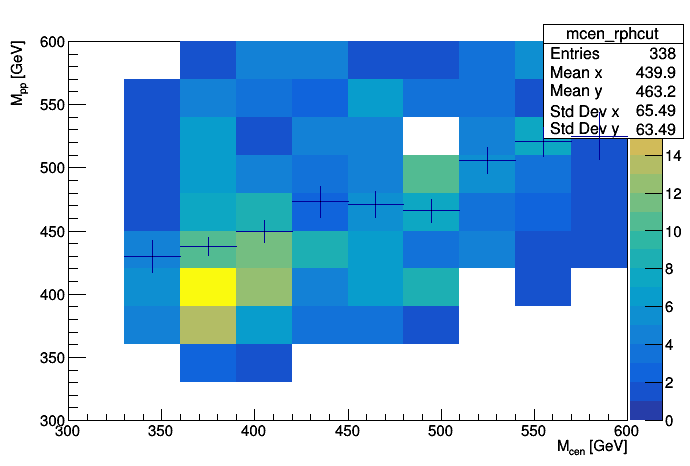
\includegraphics[width=.8\textwidth]{figures/mppsim.png}\\
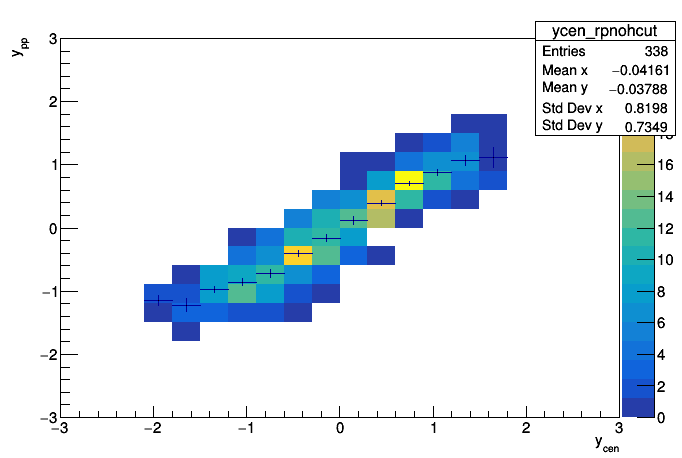
\includegraphics[width=.8\textwidth]{figures/ypp_ycen.png}
\caption{
%\FIXME{to clarify... }
%2D distributions of the mass (top) and rapidity (bottom) of the dilepton \ttbar system reconstructed using the algorithm in Ref.~\cite{1305.1878} (see text)
%for simulated exclusive \ttbar~events ($m_{cen}$, $y_{cen}$) versus the mass and rapidity of the two protons in the simulation ($m_{pp}$, $y_{pp}$). 
Distributions of the mass (top) and rapidity (bottom) of the dilepton \ttbar system as reconstructed using the algorithm in Ref.~\cite{1305.1878} (see text). 
%for the selected events in the central detector ($m_{cen}$, $y_{cen}$) versus those reconstructed from the RP tracks ($m_{RP}$, $y_{RP}$). 
2D distributions are shown for a sample of simulated exclusive \ttbar~events 
reconstructed in the central detector ($m_{cen}$, $y_{cen}$) versus the values reconstructed from the RP tracks ($m_{RP}$, $y_{RP}$).
%\FIXME{to clarify ?? The black crosses show the mean and standard deviation of the binned distribution profiles.} 
The profile of each distribution is overlaid. The black cross centers at the mean and the bars indicate the standard deviation.
}
\label{rec_kinematics_sim}
\end{figure}


\section{Background determination}
\label{sec:background}

The most important background is due to non-exclusive $\ttbar$ events superimposed to random pileup protons reconstructed in PPS. 
This background is determined with a data-driven method. 
For this purpose, a combinatorial analysis is performed, where one takes the number of tracks per event and the $\xi$ distributions in each pixel
as observed at pre-selection level where the contribution from signal events is negligible.
For each event, one generates a random number of tracks and a random $\xi$ value for each of these tracks on each side of the PPS detector. 
This allows to reconstruct random pairs of tracks from where the mass and rapidity of the candidate combinatorial pp pairs can be computed. 
If one of these combinatorial pairs is found to have a mass within the $m_{RP}\in[300,600]$\GeV range, the event is counted. 
Finally, the number of selected events is divided by the initial number of events in the sample, and the fraction of random coincidences is measured. 
We estimate the probability of random coincidences in this mass range to be $\approx$3.34\% with negligible statistical uncertainty. 
The result obtained is similar for the SF, OF, and Z peak categories.

This fake rate can be applied to all non-exclusive backgrounds and thus used to project the yields of non-exclusive \ttbar{}, tW, DY and dibosons in the signal region. 
There may be other sub-leading backgrounds that are not being considered, such as semi-exclusive \ttbar~events (where only one proton stays intact) with one pileup proton.

In addition, the events which do not pass the combinatorial pair selection (or the pair selection in data) are counted in separate categories 
that are used to normalize from data the initial estimates for \ttbar{} and DY. The latter is normalized from SF events under the Z peak.


\section{Determination of Roman Pot acceptance}
\label{sec:sigacc}

In order to estimate the acceptance of the RPs for the exclusive $pp\rightarrow p\ttbar p$ signal, a sample generated with FPMC+Herwig is used. 
A 2-dimensional distribution comparing the mass and the rapidity of the simulated $\ttbar$ system is calculated, requiring two leptons in the final state. 
Then, a cut is applied by only selecting events that fall within the expected range of the RP acceptance,
%RP acceptance expected range for $\xi$, 
\ie $0.02<\xi<0.2$. 
The distributions before and after the cut are shown in Fig.~\ref{acceptanceplots}. From these plots, one simply divides the number of surviving events by the initial number of all simulated events. The acceptance of the RPs is measured to be 1.01\%. This estimate is preliminary and could be further improved by considering that the RPs have an asymmetric acceptance between the two arms (see for example the $\xi$ distributions in Fig.~\ref{xi}) and by taking the minimum and maximum values from the $\xi$ distributions for each arm, instead of using a fixed expected range. However, the difference is not expected to be very significant.

\begin{figure}[!htp]
\centering
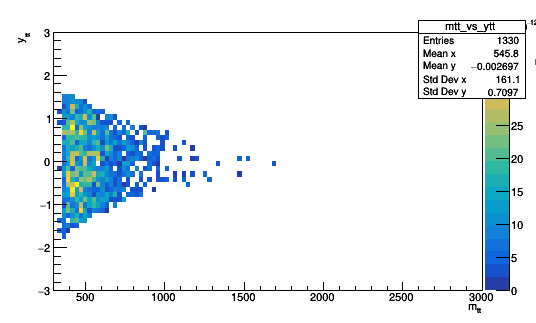
\includegraphics[width=0.49\textwidth]{figures/acceptance1.png}
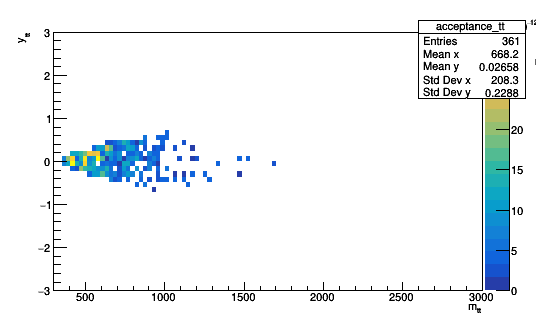
\includegraphics[width=0.49\textwidth]{figures/acceptance2.png}
\caption{2D distributions of the mass ($m_{RP}$) versus rapidity ($y_{RP}$) of the $\ttbar$ system in the signal sample, just requiring 2 leptons (left) and after requiring the tracks to be within the RP acceptance ($0.02<\xi<0.2$) (right).}
  \label{acceptanceplots}
\end{figure}

\begin{table}[ht]
\centering
\begin{tabular}{l | c | c }\hline\hline
selection step & \multicolumn{2}{c}{surviving events}  \\ \hline
Initial number of simulated events & 35920             & 100\%  \\
Events with 2 leptons              & 1330              & 3.70\%         \\
Events in RP acceptance            & 361               & 1.01\%      \\
\hline\hline
\end{tabular}
\caption{RP acceptance: number of events surviving the selection cuts and their corresponding fractions.}
\end{table}


\section{Determination of $\sigma(\exctlob)$ through a statistical analysis}
\label{stat:ana}

The final event yields, including the extrapolation of the backgrounds in the signal region using the fake rate method described in Sec.~\ref{sec:background}, are shown in Table~\ref{tab:yields_sr}. The 5 different categories share in common the selection of:

\begin{itemize}
    \item $\geq$ 2 leptons with $m_{\ell\ell}>$20\GeV;
    \item $\geq$ 1 b-jet;
    \item $m_{\ell b}<160$\GeV.
\end{itemize}

The specific requirements of the final event categories are the following:

\begin{description}
\item[SR\_OF] - $e\mu$ events with $m_{RP}\in [300,600]$ GeV and $H_T=0$\GeV;
\item[SR\_SF] - similar to SR\_OF, but for same-flavour events outside the Z peak;
\item[\ttbar CR\_OF] - $e\mu$ events failing the $m_{RP}\in [300,600]$\GeV cut;
\item[\ttbar CR\_SF] - similar to \ttbar CR\_OF, but for same-flavour events outside the Z peak;
\item[dyCR] - similar to \ttbar CR\_SF, but for same-flavour events inside the Z peak.

\end{description}

In the following, we perform a combined fit of the event yields observed in each category.

\begin{table}[!htp]
\centering
%\begin{tabular}{|
%>{\columncolor[HTML]{EFEFEF}}l |c|c|}
%
\begin{tabular}{l | c|c}
\hline\hline
%\multicolumn{1}{|c|}{\cellcolor[HTML]{C0C0C0}} & \cellcolor[HTML]{EFEFEF}SR\_SF & \cellcolor[HTML]{EFEFEF}SR\_OF\\ 
%\multicolumn{1}{|c|} & SR\_SF & SR\_OF\\ 
Process & SR\_SF & SR\_OF \\
\hline
inclusive \ttbar		& 1172	& 1460	\\
DY				& 1742	& 97		\\
others			& 30		& 34		\\ \hline
total				& 2944	& 1591	\\ \hline
data				& 2538	& 1130	\\ \hline\hline
\end{tabular}
\caption{Yields in the signal region for different background contributions and for those observed in data.}
\label{tab:yields_sr}
\end{table}

\begin{table}[!htp]
\centering
%\begin{tabular}{|
%>{\columncolor[HTML]{EFEFEF}}l |c|c|c|}
%
\begin{tabular}{l | c|c|c}
\hline\hline
%\multicolumn{1}{|c|}{\cellcolor[HTML]{C0C0C0}} & \cellcolor[HTML]{EFEFEF}\ttbar CR\_SF & \cellcolor[HTML]{EFEFEF}\ttbar CR\_OF & \cellcolor[HTML]{EFEFEF}dyCR \\ 
Process & \ttbar CR\_SF & \ttbar CR\_OF &  dyCR \\
\hline
inclusive \ttbar & {\bf 415937}                         & {\bf 519492}                         & 114783                     \\
DY                                             & 271583                         & 17395                          & {\bf 2863390}  \\
others                                         & 9962                           & 12180                          & 11756               \\ \hline
total                                          & 697483                         & 549068                         & 2989929          \\ \hline
data                                      & 903621                         & 550805                         & 3759454              \\ \hline\hline
\end{tabular}
\caption{Yields in the control regions for different background contributions and those observed in data.}
\label{tab:yields_cr}
\end{table}


\subsection{Method employed in the statistical analysis}
\label{subsec:statanamethod}

The number of events observed in the signal and control regions can be analyzed to set limits on the production cross section of $\exctlob$. In order to do it we parametrize the total number of events expected in a single category  as follows:

\begin{equation}
N_{\rm exp}=N_{\rm exp}(\exctlob)+f\cdot\left[N_{\rm exp}(\ttbar)+N_{\rm exp}({\rm tW})+N_{\rm exp}({\rm DY})+N_{\rm exp}({\rm others})\right]
\label{eq:nexp}    
\end{equation}

where $f$ is the probability that a non-exclusive event passes the selection of the RPs due to combinatorial tracks. In Eq.~\ref{eq:nexp} we assume that there is no additional exclusive process which may contribute in the selected regions.
The CRs for \ttbar~ and DY are used to normalized the initial expectations based on simulation. We thus employ  $\mu_\ttbar$ ($\mu_{\rm DY}$) as scaling factors of the initial expectations for \ttbar (DY), \ie:

\begin{equation}
N_{\rm exp}(b)=\mu_b \cdot N_{\rm exp}^{\rm MC}(b)
\label{eq:bkgscaling}
\end{equation}

where b=\ttbar,DY and $N_{\rm exp}^{\rm MC}(b)$ is the expectation from simulation which includes the theory cross section, the integrated luminosity, and the corrections for the simulated efficiency with data-to-MC scale factors.
Other processes in Eq.~\ref{eq:nexp} will float constrained according to the estimated uncertainties.
The expectations for the signal are written as a product of the following factors:

\begin{equation}
N_{\rm exp,c}(\exctlob)=A\cdot L \cdot \varepsilon_{\rm c} \cdot \sigma(\exctlob)
\label{eq:signalscaling}
\end{equation}

where c=SF,OF is the event category, $A$ is the acceptance at generator level for the selection of two leptons and an invariant mass of the outgoing protons in the PPS detector acceptance, $L$ is the total integrated luminosity, $\varepsilon_{\rm c}$ is the selection efficiency, and $\sigma_\exctlob$ is the cross section. Given that the selection criteria differ slightly in the SF and OF categories, the efficiency factors in Eq.~\ref{eq:signalscaling} are computed separately for each category.
With these definitions in hand, we can maximize the following likelihood as function of $\sigma_\exctlob$

\begin{equation}
\mathcal{L}=\prod_{k=1}^{N}\mathcal{P}_{\rm oisson}(N_{\rm obs}|N_{\rm exp})\cdot \prod_{m=1}^{M} f(\theta_k)
\label{eq:ll}
\end{equation}

where the first product runs over the $N$ categories in which events are counted, and the second product runs over $M$ nuisance parameters which encode the relative uncertainty of the parameters employed to parametrize the expectations $N_{\rm exp}$. The PDF $f(\theta_k)$ is taken as a log-normal function. The implementation of Eqs~\ref{eq:nexp}-~\ref{eq:ll} is made in RooStats, using the Higgs Combine Tool.


%%
%%
%%
\subsection{Summary of the inputs to the statistical analysis}
\label{subsec:statinputsummary}

Table~\ref{tab:sig_summary} summarizes the values used for the acceptance, efficiency, 
and the number of expected events corresponding to the integrated luminosity in which the data are analysed.
The systematic uncertainties considered in the fit are listed in Table~\ref{tab:systs}.

\begin{table}[!htp]
\centering
\begin{tabular}{l|c|c}
\hline\hline
 & SF & OF \\ \hline
Signal acceptance                              & \multicolumn{2}{c}{0.0101}   	        \\ \hline
Selection efficiency ($m_{\ell b}<160\GeV$)	& 0.345	& 0.428		\\ \hline
N (luminosity * acc. * eff.)                   		& 65.055	& 80.697		\\ \hline\hline
\end{tabular}
\caption{Summary of the inputs to the statistical analysis. 
Signal acceptance, the selection efficiency in the signal region ($m_{\ell b}<160\GeV$), and the number of expected events. 
Numbers are shown for same-flavour (SF) and opposite-flavour (OF) categories.}
\label{tab:sig_summary}
\end{table}

\begin{table}[ht]
\centering
\begin{tabular}{c|c|c}
\hline\hline
Uncertainty                 & Value & It affects                     \\ \hline
Luminosity                  & 2.7\% & all processes               \\
$\sigma_{\rm inclusive~\ttbar}$        & 5.1\% & inclusive $\ttbar$ (SR and CR)    \\
$\sigma_{\rm others}$           & 30\%  & others                      \\
DY uncertainty              & 30\%  & Drell-Yan                   \\
Fake rate                   & 5\%   & all processes except signal \\
Lepton selection efficiency & 3\%   & all processes               \\ \hline\hline
\end{tabular}
\caption{Systematic uncertainties used in the analysis.}
\label{tab:systs}
\end{table}


\subsection{Results}
\label{subsec:results}

Using the Higgs Combine Tool with the inputs listed in Section~\ref{subsec:statinputsummary}, one can obtain the likelihood plots shown in Fig.~\ref{fig:likelihood}. It is then possible to get an asymptotic upper limit on the exclusive \ttbar cross section: $\sigma <900 \substack{+360 \\ -253}$~fb (68\% confidence level), or $900 \substack{+415 \\ -788}$~fb (95\% confidence level).

\begin{figure}[ht]
\centering
%\begin{subfigure}{.8\columnwidth}
%  \centering
  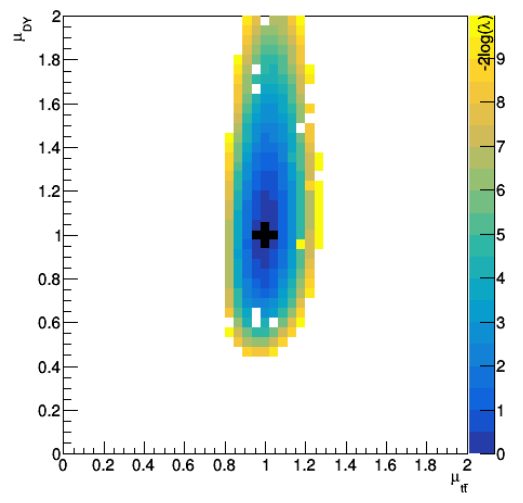
\includegraphics[width=.49\linewidth]{figures/likelihood_contour.png}
%  \subcaption{}
%\end{subfigure}
%
%\begin{subfigure}{.8\columnwidth}
%  \centering
  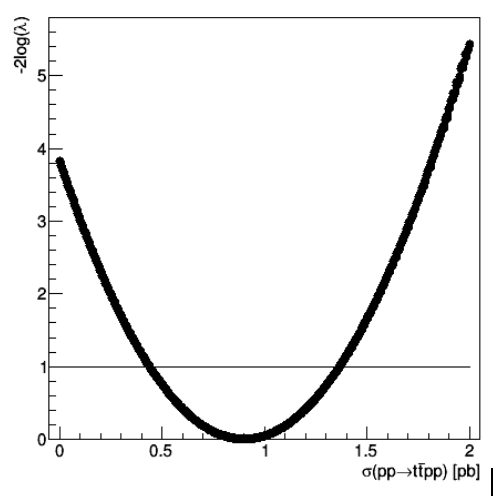
\includegraphics[width=.49\linewidth]{figures/likelihood_scans.png}
%  \subcaption{}
%\end{subfigure}
\caption{
{\it Left:} Contour of the likelihood for the scale factors for inclusive $\ttbar$ ($\mu_\ttbar$) and DY ($\mu_{DY}$) processes fitted using dedicated control regions. 
The black cross marks the fitted values. 
{\it Right:} Likelihood scan results for the expected signal for a cross section of $\sigma=900$~fb. The line intersects the likelihood at the boundaries of the 68\%CL. }
\label{fig:likelihood}
\end{figure}


\section{Conclusions}
\label{sec:conclusions}

We analysed the 2017 data searching for  exclusive \ttbar~production in the dilepton final state. 
An inclusive selection for two leptons and at least one b jet is studied and the background estimated. 
Signal discrimination variables are studied based on a dedicated simulation of 
$pp\rightarrow p\gamma\gamma p\rightarrow p \ttbar p$.
The estimated upper limit on the production cross section of exclusive \ttbar{} production is 900~fb.


% >> acknowledgments (for journal papers only)
% The latest version of the acknowledgments will be included from https://twiki.cern.ch/twiki/bin/viewauth/CMS/Internal/PubAcknow as of the date of submission.
%\begin{acknowledgments}
%
%\end{acknowledgments}

%% **DO NOT REMOVE BIBLIOGRAPHY**
\bibliography{auto_generated}   % will be created by the tdr script.
 \renewcommand*{\chaptermark}[1]{}
%% examples of appendices. **DO NOT PUT \end{document} at the end
%\clearpage
\end{document}

